\documentclass[11pt,a4paper]{article}

% ---------------------------------------------------------------
% Packages
% ---------------------------------------------------------------
\usepackage[utf8]{inputenc}
\usepackage[T1]{fontenc}
\usepackage{lmodern}
\usepackage[margin=1in]{geometry}
\usepackage{amsmath, amssymb, amsthm, mathtools}
\usepackage{graphicx}
\usepackage{booktabs}
\usepackage{multirow}
\usepackage{array}
\usepackage[expansion=false]{microtype}
\usepackage{listings}
\usepackage{xcolor}
\usepackage{textcomp}
\usepackage{enumitem}
\usepackage{tabularx}
\usepackage{hyperref}
\hypersetup{colorlinks=true, linkcolor=blue!50!black, citecolor=blue!50!black, urlcolor=blue!50!black}

\graphicspath{{figures/}}
\setlength{\emergencystretch}{2em}

\lstdefinestyle{pystyle}{
    language=Python,
    basicstyle=\ttfamily\footnotesize,
    keywordstyle=\color{blue},
    commentstyle=\color{gray},
    stringstyle=\color{teal},
    showstringspaces=false,
    breaklines=true,
    frame=single,
    tabsize=4
}

% ---------------------------------------------------------------
% Theorem environments and macros
% ---------------------------------------------------------------
\theoremstyle{plain}
\newtheorem{theorem}{Theorem}[section]
\newtheorem{proposition}[theorem]{Proposition}
\newtheorem{lemma}[theorem]{Lemma}
\theoremstyle{definition}
\newtheorem{definition}[theorem]{Definition}
\newtheorem{remark}[theorem]{Remark}

\newcommand{\dd}{\mathrm{d}}
\newcommand{\E}{\mathbb{E}}
\newcommand{\Q}{\mathbb{Q}}
\newcommand{\R}{\mathbb{R}}
\newcommand{\bp}{\,\mathrm{bp}}
\newcommand{\eur}{\text{\texteuro}}
\newcommand{\estr}{\text{\texteuro STR}}
\DeclareMathOperator*{\argmin}{arg\,min}


\title{\textbf{Construction of the \texteuro STR Curve:\\
OIS Bootstrap, ECB Meeting Dates and Proxy Quotes}}
\author{\textbf{Elias Benguedda}}
\date{October 2026}

\begin{document}

\maketitle

\begin{abstract}
This paper builds the \estr{} discounting curve, the risk-free curve of the euro area and the discount curve of collateralized euro derivatives. It extends the single-curve framework of the yield curve paper of this portfolio. We recall the definition of the \estr{} fixing and the cash flows of an overnight indexed swap (OIS), with daily compounding and market conventions (ACT/360, TARGET2 calendar, spot lag, payment lag), and we check them by rebuilding the ECB compounded \estr{} index from 1,797 daily fixings. The curve is bootstrapped from public data~\cite{data}; since \estr{} OIS quotes are not free, they are replaced by proxy quotes built from the ECB AAA government curve, shifted by the average gap between the AAA curve and the realized \estr{} ($4.9\bp$).

A standard bootstrap, with one pillar per OIS, reprices the 25 quotes to machine precision and matches QuantLib to $2\times10^{-8}\bp$, but its overnight forwards jump at the OIS maturities or spread the policy decisions over several months. The short end is therefore rebuilt with pillars on the ECB effective dates, which gives piecewise constant overnight forwards and a readable policy path: on the proxy quotes, about $71\bp$ of hikes, i.e.\ 2.8 moves of $25\bp$, are priced over 18 months. The two constructions agree on discounting within $2.3\bp$ of zero rate, but differ by $3\bp$ on the forward between two meetings. The implied path depends strongly on the proxy: one standard deviation of the AAA--OIS basis moves the number of hikes priced in one year from 2.4 to 3.1. Finally, the par-point risk of a forward-starting OIS shows that flat-forward curves give additive bucketed risks, whereas monotone convex does not. This paper is linked to my GitHub, which can be found on my portfolio\footnote{\url{https://portfolio-eliasbenguedda.fr}}, and all scripts are available in the same repository.
\end{abstract}

\clearpage

\tableofcontents
\newpage

% ===============================================================
\section{Introduction}
\label{sec:intro}
% ===============================================================

\subsection{Motivation}
To price vanillas, exotics, structured products, we need rates and so, first, we need to build a discount curve. Collateralized derivatives are discounted at the rate paid on the collateral, which for euro trades is the overnight rate \estr{} (Euro Short-Term Rate). Each IBOR tenor (EURIBOR 3M, 6M) has its own projection curve, and the basis spreads between them are material.

\estr{} is published by the ECB since 2 October 2019 and replaced EONIA (EONIA $=$ \estr{} $+\,8.5\bp$ until its discontinuation on 3 January 2022)\footnote{The equivalent of \estr{} in the US is SOFR, for the UK it is SONIA}. Its OIS market is liquid from one week to 30 years. Building this curve is therefore the first step of any euro rates pricer:
\begin{enumerate}[label=(\roman*)]
    \item a \emph{discount curve} for collateralized cash flows;
    \item a \emph{forward curve} of the overnight rate, whose short end reflects the expected ECB decisions;
    \item the base on which the EURIBOR projection curves are built (Section~\ref{sec:next-steps}).
\end{enumerate}

The \estr{} curve is the risk-free zero-coupon curve of the euro area, i.e.\ a set of discount factors $P(0,t)$, from which zero rates and forwards are derived. Compared with the zero curve of the yield curve paper, it has three specificities: the underlying rate is an overnight rate compounded daily, its short end moves in steps with the ECB decisions, and the instruments follow precise market conventions (calendar, spot lag, payment lag). Since the \estr{} curve discounts the \estr{} flows themselves, the single-curve framework is exact here.

We must note that because OIS data is not available for free on internet we will use a proxy. We will take the AAA yield curve provided by the ECB as an approximation of the \estr{} curve, corrected by the average gap between the two curves (Section~\ref{sec:proxy}). The construction is independent of this choice: with market quotes, only the input file changes.

\subsection{Organization of the paper}
Section~\ref{sec:prelim} defines the \estr{} fixing, the OIS cash flows and the conventions, and checks them against the ECB compounded index. Section~\ref{sec:data} describes the data. Section~\ref{sec:proxy} builds the proxy OIS quotes from the AAA curve. Section~\ref{sec:standard} performs a standard bootstrap, used as a baseline and to validate the instruments. Section~\ref{sec:meetings} builds the short end on the ECB meeting dates and reads the implied policy path. Section~\ref{sec:risk} studies the par-point risk. Section~\ref{sec:limits} discusses the limitations, Section~\ref{sec:next-steps} lists next steps and Section~\ref{sec:conclusion} concludes. Appendix~\ref{app:code} gives excerpts of the Python implementation and Appendix~\ref{app:notation} the notation.

\clearpage
% ===============================================================
\section{The \texteuro STR Rate and Overnight Indexed Swaps}
\label{sec:prelim}
% ===============================================================

\subsection{The \texteuro STR fixing}
\estr{} is computed by the ECB from the overnight unsecured borrowing transactions of euro area banks with financial counterparties~\cite{ecbestr}. It is a volume-weighted trimmed mean: the transactions are ranked by rate, the top and bottom 25\% of the volume are removed, and the remaining 50\% are averaged with volume weights. It is published at 8:00 CET on the next TARGET2 business day for the previous day, together with the volume, the number of transactions and of reporting banks, and the share of the five largest banks; a contingency procedure applies when the data are insufficient.

The rate is an annualized simple rate on the ACT/360 basis. Investing one euro overnight from business day $d_i$ to the next business day $d_{i+1}$ pays $1+r_i\,n_i/360$, where $n_i$ is the number of calendar days (3 over a weekend).

\subsection{Compounded \texteuro STR}
Over an accrual period $[T_s,T_e]$ with business days $d_0=T_s<d_1<\dots<d_N=T_e$, the floating coupon of an OIS is the daily compounded rate
\begin{equation}
    R(T_s,T_e)=\frac{360}{D}\left(\prod_{i=0}^{N-1}\Bigl(1+r_i\,\frac{n_i}{360}\Bigr)-1\right),\qquad D=\sum_{i=0}^{N-1}n_i.
    \label{eq:compounded}
\end{equation}
Under the risk-neutral measure associated with \estr{} discounting, $\prod_i(1+r_in_i/360)$ is the value at $T_e$ of one euro rolled overnight from $T_s$. Its present value is therefore $P(0,T_s)$, so the floating leg of a period is worth
\begin{equation}
    \text{PV}_{\text{float}}=P(0,T_s)-P(0,T_e),
    \label{eq:float-leg}
\end{equation}
without any convexity or timing adjustment, provided the payment date is $T_e$. With a payment lag, the period paid at $p_i>T_e$ is worth $P(0,p_i)\bigl(P(0,T_s)/P(0,T_e)-1\bigr)$. Since the lag applies to both legs, its effect on the par rate is tiny: on our curve, removing the one-day lag changes the par rates by less than $0.0011\bp$ up to 30 years. It is nevertheless kept, so that the schedules match the market ones exactly (Section~\ref{sec:validation}).

\subsection{OIS par rate}
A spot-starting OIS of maturity $T$ exchanges annual fixed payments $K\,\delta_j$ (ACT/360) against the compounded \estr{}~\eqref{eq:compounded}. With periods $[s_i,e_i]$ paid at $p_i$, the par rate is
\begin{equation}
    K=\frac{\sum_iP(0,p_i)\bigl(P(0,s_i)/P(0,e_i)-1\bigr)}{\sum_i\tau_i\,P(0,p_i)},\qquad \tau_i=\frac{e_i-s_i}{360},
    \label{eq:ois-par}
\end{equation}
which reduces to the formula of the yield curve paper without payment lag: $S(T)=\bigl(P(0,T_0)-P(0,T_n)\bigr)/\sum_j\delta_jP(0,t_j)$, $T_0$ being the spot date. OIS of maturity up to one year have a single payment at maturity: $S(T)\,\delta=P(0,T_0)/P(0,T)-1$, the same equation as a deposit.

\subsection{Conventions}
\begin{table}[htbp]
\centering
\begin{tabular}{@{}ll@{}}
\toprule
Item & \estr{} OIS convention \\
\midrule
Calendar & TARGET2 \\
Spot lag & $T+2$ business days \\
Day count (both legs) & ACT/360 \\
Fixed leg frequency & annual (short front stub; single payment up to 1 year) \\
Business day convention & modified following \\
Payment lag & 1 business day \\
Fixing publication & $T+1$, 8:00 CET \\
ECB decisions & effective on the Wednesday after the meeting \\
Model time & ACT/365 from the valuation date \\
\bottomrule
\end{tabular}
\caption{Conventions used in the implementation. The OIS schedules coincide date by date with those of QuantLib's \texttt{Estr} OIS (Section~\ref{sec:validation}).}
\label{tab:conventions}
\end{table}

\subsection{Conventions check: rebuilding the ECB compounded index}
The ECB publishes, with the fixings, a compounded \estr{} index $I_t=100\prod_k(1+r_kn_k/360)$ (base 100 on 1 October 2019) and the compounded averages over 1 week to 12 months. Rebuilding them from the daily fixings checks the TARGET calendar (which business days have a fixing, and how many calendar days each fixing covers) and the ACT/360 day count. Over the 1,797 days of the sample, the rebuilt index differs from the ECB one by at most $5\times10^{-9}$, and the averages agree to the fifth decimal (Table~\ref{tab:index-check}), which is the rounding of the published values (8 decimals for the index, 5 for the averages).

\begin{table}[htbp]
\centering
\small
\begin{tabular}{@{}lrrr@{}}
\toprule
On 2026-10-06 & Rebuilt from fixings & ECB & Difference \\
\midrule
Index & 109.935 & 109.935 & $-5.3\times10^{-10}$ \\
1M average (\%) & 2.34817 & 2.34817 & $4.1\times10^{-6}$ \\
3M average (\%) & 2.24781 & 2.24781 & $3.0\times10^{-6}$ \\
6M average (\%) & 2.12073 & 2.12073 & $-4.4\times10^{-6}$ \\
12M average (\%) & 2.04256 & 2.04256 & $-3.8\times10^{-7}$ \\
\bottomrule
\end{tabular}
\caption{ECB compounded \estr{} index and averages rebuilt from the daily fixings.}
\label{tab:index-check}
\end{table}

These averages are realized, backward-looking rates. The curve is about the forward-looking expectation of the same compounded rates, which is what OIS quotes give; the index is used again in Section~\ref{sec:proxy} to measure the gap between the AAA curve and the \estr{}.

\clearpage
% ===============================================================
\section{Data}
\label{sec:data}
% ===============================================================

\subsection{\texteuro STR fixings and the ECB corridor}

The data are downloaded from the ECB Data Portal~\cite{ecbdata}: 1,797 daily \estr{} fixings from 1 October 2019 to 6 October 2026, the ECB key rates, the meeting calendar and the AAA government curve. The valuation date is 5 October 2026, with an \estr{} of $2.438\%$ and a deposit facility rate of $2.50\%$.

\begin{figure}[htbp]
    \centering
    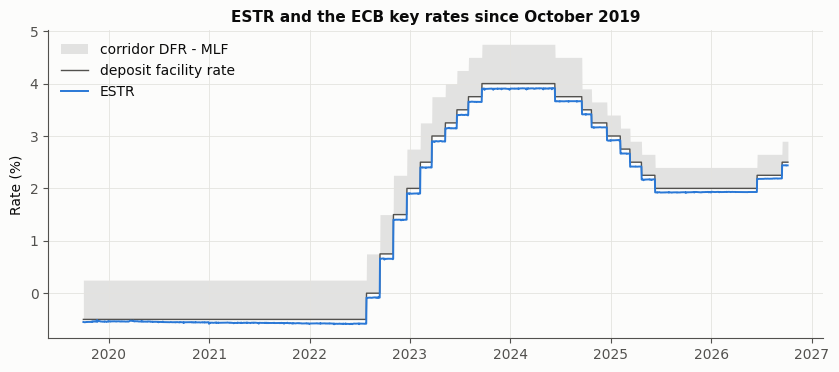
\includegraphics[width=0.7\textwidth]{estr_fixings.png}
    \caption{\estr{} fixings and ECB key rates from October 2019 to October 2026.}
    \label{fig:fixings}
\end{figure}

Figure~\ref{fig:fixings} also shows the ECB key rates. The deposit facility rate (DFR) is the rate the ECB pays to banks on their overnight deposits at the central bank. In the current regime of excess liquidity it is the main policy rate: a bank has no reason to lend overnight below the DFR, since it can deposit its cash at the ECB without any risk. The marginal lending facility rate (MLF), at which banks can borrow overnight from the ECB against collateral, is the ceiling of the corridor, and the main refinancing rate (MRO) lies between the two. The corridor DFR--MLF\footnote{DFR--MLF: Deposit Facility Rate -- Marginal Lending Facility Rate} therefore bounds the overnight rates of the banks.

The \estr{} is nevertheless \emph{below} the DFR, because it includes the transactions with non-bank lenders (money market funds, insurers, public institutions) that have no access to the deposit facility and accept to lend to banks below the DFR.

\subsection{The \texteuro STR -- DFR spread}
Table~\ref{tab:spread} gives the spread between the \estr{} and the DFR by year. It is negative, between $-4\bp$ and $-10\bp$, and very stable within a year: its standard deviation is below $1\bp$, while the dispersion of the transactions around the fixing (25--75 percentile range) is of $3$ to $6\bp$. The spread widened until 2023 with the excess liquidity and narrows since then as the liquidity is withdrawn ($-6.7\bp$ on average in 2026, $-6.3\bp$ over the last three months).

\begin{table}[htbp]
\centering
\small
\begin{tabular}{@{}lrrrrr@{}}
\toprule
Year & Mean (bp) & Std (bp) & Min (bp) & Max (bp) & 25--75 range (bp) \\
\midrule
2019 & $-4.2$ & 0.7 & $-5.5$ & $-1.1$ & 3.9 \\
2020 & $-4.7$ & 0.9 & $-8.3$ & $-2.2$ & 3.4 \\
2021 & $-6.8$ & 0.5 & $-9.0$ & $-5.8$ & 4.3 \\
2022 & $-8.6$ & 0.8 & $-11.0$ & $-7.2$ & 3.8 \\
2023 & $-10.0$ & 0.4 & $-12.0$ & $-9.3$ & 6.0 \\
2024 & $-8.9$ & 0.5 & $-11.3$ & $-8.1$ & 4.9 \\
2025 & $-7.8$ & 0.5 & $-9.4$ & $-6.6$ & 4.9 \\
2026 & $-6.7$ & 0.3 & $-7.4$ & $-5.8$ & 4.3 \\
\bottomrule
\end{tabular}
\caption{\estr{} $-$ DFR spread by year, and mean 25--75 percentile range of the transactions.}
\label{tab:spread}
\end{table}

This stability is what makes the policy path the backbone of the short end of the curve: between two meetings the \estr{} is almost constant, and it jumps on the effective date of each decision (Section~\ref{sec:meetings}).

\subsection{AAA government curve (source of the proxy quotes)}

The data are in the \texttt{ECB\_AAA\_YieldCurve.csv} file, which also contains the Svensson parameters published by the ECB. Table~\ref{tab:quotes} gives the spot rates of the valuation date.

\begin{table}[htbp]
\centering
\small
\begin{tabular}{@{}lrlrlr@{}}
\toprule
Tenor & Rate (\%) & Tenor & Rate (\%) & Tenor & Rate (\%) \\
\midrule
3M & 2.5305 & 4Y & 3.1072 & 10Y & 3.5020 \\
6M & 2.6743 & 5Y & 3.1674 & 12Y & 3.6079 \\
9M & 2.7780 & 6Y & 3.2349 & 15Y & 3.7237 \\
1Y & 2.8527 & 7Y & 3.3051 & 20Y & 3.8178 \\
2Y & 2.9971 & 8Y & 3.3745 & 25Y & 3.8229 \\
3Y & 3.0555 & 9Y & 3.4406 & 30Y & 3.7722 \\
\bottomrule
\end{tabular}
\caption{ECB AAA government spot rates (continuously compounded) on 2026-10-05.}
\label{tab:quotes}
\end{table}

\begin{figure}[htbp]
    \centering
    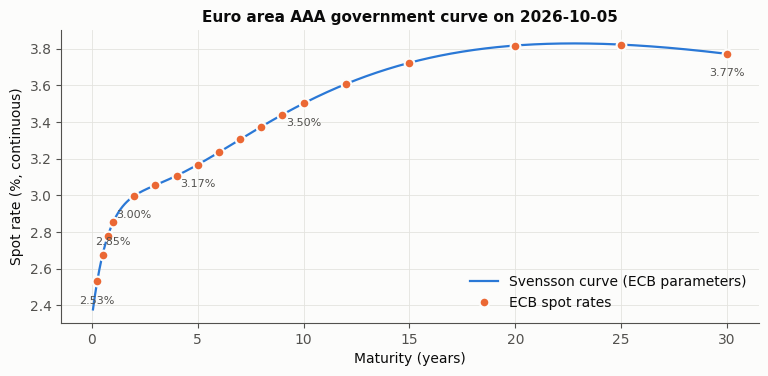
\includegraphics[width=0.7\textwidth]{ois_quotes.png}
    \caption{Euro area AAA government curve on 2026-10-05: Svensson curve and ECB spot rates.}
    \label{fig:quotes}
\end{figure}

\clearpage

\subsection{ECB monetary policy meetings}

We also imported the list of the Governing Council monetary policy meeting dates. This data is important because, as can be seen on the \estr{} fixings, the rate moves in a discretionary manner: rates are decided during the ECB meetings, and the new rates are effective on the Wednesday of the following week, at the start of the reserve maintenance period. After the valuation date, the calendar contains 18 effective dates up to 13 December 2028, 16 of them within two years; the first ones are 4 November 2026, 23 December 2026, 10 February 2027 and 24 March 2027.

\subsection{From the \estr{} fixing to a curve}

One may wonder how a whole curve can be built from a single overnight rate.
The \estr{} fixing only gives one point: the overnight rate of today. The
information on future rates comes from overnight indexed swaps. An OIS of
maturity $T$ exchanges a fixed rate against the \estr{} compounded up to $T$,
so its par rate reflects the path of the \estr{} that the market expects until
$T$, plus a term premium. Since the \estr{} closely tracks the ECB deposit
facility rate, this expected path is mainly the expected path of monetary
policy. Bootstrapping the OIS par rates then gives the discount factors of the
\estr{} curve, and hence its zero rates and forwards. In this paper, market OIS
quotes are replaced by the proxy quotes of Section~\ref{sec:proxy}, so the
curve reflects the expectations embedded in the AAA government curve rather
than those of the OIS market.

\clearpage
% ===============================================================
\section{Proxy OIS Quotes}
\label{sec:proxy}
% ===============================================================

\subsection{Svensson curve}

The ECB fits the Svensson model~\cite{svensson} on the prices of the AAA-rated euro area government bonds, and publishes in \texttt{ECB\_AAA\_YieldCurve.csv} both the fitted parameters and the spot rates of the fitted curve. The continuously compounded spot rate of maturity $T$ is
\begin{equation}
z_{\mathrm{AAA}}(T) = \beta_0 + \beta_1 \left( \frac{1 - e^{-T/\tau_1}}{T/\tau_1} \right) + \beta_2 \left( \frac{1 - e^{-T/\tau_1}}{T/\tau_1} - e^{-T/\tau_1} \right) + \beta_3 \left( \frac{1 - e^{-T/\tau_2}}{T/\tau_2} - e^{-T/\tau_2} \right).
\label{eq:svensson}
\end{equation}
The formula defines the curve at every maturity, not only at the published tenors, which is what the proxy needs: its instantaneous forward $f_{\mathrm{AAA}}(0,T)=\partial_T\bigl(T\,z_{\mathrm{AAA}}(T)\bigr)$ is available in closed form, and par rates can be computed on any dated schedule.

\begin{table}[htbp]
\centering
\footnotesize
\setlength{\tabcolsep}{4pt}
\begin{tabular}{@{}lrrr@{\hspace{1.5em}}lrrr@{}}
\toprule
Tenor & ECB spot (\%) & Svensson (\%) & Diff.\ (bp) & Tenor & ECB spot (\%) & Svensson (\%) & Diff.\ (bp) \\
\midrule
3M  & 2.530476 & 2.530476 & $-3.8\times10^{-10}$ & 6Y  & 3.234878 & 3.234878 & $7.8\times10^{-9}$ \\
6M  & 2.674286 & 2.674286 & $3.2\times10^{-9}$   & 7Y  & 3.305120 & 3.305120 & $6.2\times10^{-9}$ \\
9M  & 2.778026 & 2.778026 & $3.4\times10^{-9}$   & 8Y  & 3.374513 & 3.374513 & $7.7\times10^{-9}$ \\
1Y  & 2.852743 & 2.852743 & $4.9\times10^{-9}$   & 9Y  & 3.440616 & 3.440616 & $9.0\times10^{-9}$ \\
2Y  & 2.997130 & 2.997130 & $5.3\times10^{-9}$   & 10Y & 3.501981 & 3.501981 & $3.9\times10^{-9}$ \\
3Y  & 3.055535 & 3.055535 & $2.7\times10^{-9}$   & 12Y & 3.607910 & 3.607910 & $8.1\times10^{-9}$ \\
4Y  & 3.107177 & 3.107177 & $2.2\times10^{-9}$   & 15Y & 3.723674 & 3.723674 & $3.1\times10^{-9}$ \\
5Y  & 3.167448 & 3.167448 & $-5.0\times10^{-10}$ & 20Y & 3.817818 & 3.817818 & $5.0\times10^{-9}$ \\
    &          &          &                      & 25Y & 3.822865 & 3.822865 & $2.3\times10^{-10}$ \\
    &          &          &                      & 30Y & 3.772198 & 3.772198 & $7.7\times10^{-10}$ \\
\bottomrule
\end{tabular}
\caption{ECB AAA spot rates (continuously compounded) on 2026-10-05 against the Svensson formula evaluated with the ECB parameters
($\beta_0=1.7202$, $\beta_1=0.6117$, $\beta_2=1.9283$, $\beta_3=6.7187$, $\tau_1=0.9659$, $\tau_2=13.6006$). Difference = ECB $-$ Svensson, in basis points.}
\label{tab:svensson-check}
\end{table}

Since the published spot rates are themselves computed by the ECB from the fitted curve, Table~\ref{tab:svensson-check} is not a test of the model but of our implementation: the differences, below $10^{-8}\bp$, are the rounding of the published values, and they confirm the parameter conventions (rates in percent, $\tau_1,\tau_2$ in years). Two limits of the AAA curve should be kept in mind: it is itself the output of a smooth fit, which does not pass exactly through the bond prices, and no AAA bond is shorter than about one year, so its short end is an extrapolation.

\subsection{Government vs OIS basis}

The AAA curve is not the \estr{} curve: the two rates do not carry the same risk and are not used for the same purpose. The ECB AAA curve is fitted on the central government bonds of the AAA-rated euro area countries, mainly Germany and the Netherlands. These bonds are the euro area safest assets: they are used as collateral and as a store of value, so their yield contains a convenience and liquidity premium, and it also depends on the supply of public debt and on repo specialness. An OIS, on the other hand, only exchanges a fixed rate against the compounded overnight rate and carries almost no credit or liquidity premium. The difference between the two curves, the government--OIS basis, therefore depends on the maturity and on the market regime, and it can change sign. During stress periods, the flight to quality pushes AAA yields below OIS rates.

Since \estr{} OIS quotes are not available, the basis cannot be read directly from the market. We measure it ex post, by replacing the OIS rate with what the \estr{} actually did: on each date $t$, the 3-month AAA spot rate is compared with the \estr{} compounded over the following three months, computed from the ECB index $I_t$,
\begin{equation}
    b(t)=z_{\mathrm{AAA}}(t;3\mathrm{M})-\frac{1}{\tau}\ln\frac{I_{t+3\mathrm{M}}}{I_t},
    \label{eq:basis}
\end{equation}
where both rates are continuously compounded and $\tau$ is the ACT/365 length of the period. Figure~\ref{fig:basis} shows the result.

\begin{figure}[htbp]
    \centering
    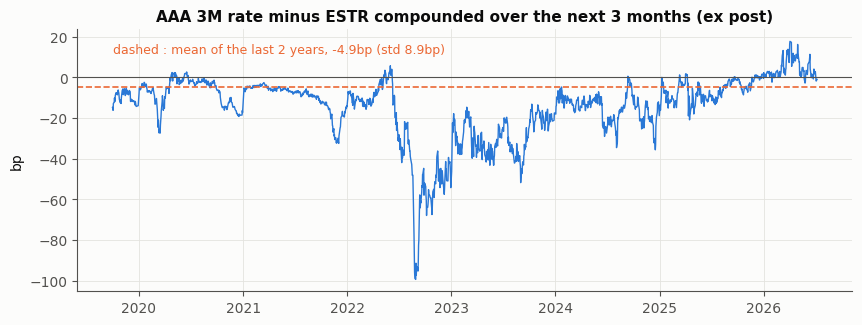
\includegraphics[width=0.7\textwidth]{aaa_ois_basis.png}
    \caption{AAA 3M rate minus \estr{} compounded over the next 3 months (ex post).}
    \label{fig:basis}
\end{figure}

The basis is a few basis points below zero in calm periods, but it falls to about $-100\bp$ in 2022. This measure must be read with care, for three reasons:
\begin{itemize}
    \item it mixes the basis with forecast errors: the realized \estr{} includes the policy surprises, and in 2022 the ECB hiked much faster than expected, so most of the 2022 trough is an error of anticipation, not a difference of risk;
    \item no AAA bond is as short as three months, so the 3-month point of the Svensson curve is an extrapolation: the basis is measured on the least reliable part of the AAA curve;
    \item it is only measured at three months, whereas the basis depends on the maturity.
\end{itemize}
Over the last two years, the basis has a mean of $\bar b=-4.9\bp$ and a standard deviation of $8.9\bp$. The mean is used to build the proxy quotes, and the standard deviation gives the order of magnitude of their uncertainty (Section~\ref{sec:proxy-sensitivity}).

\subsection{Proxy forward curve and quotes}

The proxy instantaneous forward curve is built in two parts:
\begin{equation}
    f^{\mathrm{proxy}}(0,t)=
    \begin{cases}
        r_{ON}, & t<E_1,\\[1mm]
        f_{\mathrm{AAA}}(0,t)-\bar b, & t\ge E_1,
    \end{cases}
    \label{eq:proxy-fwd}
\end{equation}
where $r_{ON}=365\ln\bigl(1+r_0/360\bigr)$ is today's \estr{} fixing $r_0$ converted to a continuously compounded ACT/365 rate, $E_1$ is the first ECB effective date (4 November 2026) and $f_{\mathrm{AAA}}(0,t)$ is the instantaneous forward of the Svensson curve~\eqref{eq:svensson}. Before $E_1$ no decision can change the \estr{}, so the forward is set to today's fixing. Beyond, the proxy is the AAA forward shifted up by $-\bar b=4.9\bp$, the average gap between the realized \estr{} and the AAA curve. The forward jumps at $E_1$, which is consistent with a policy decision on that date. The integrated forward $y(t)=\int_0^tf^{\mathrm{proxy}}$ is computed on a fine grid (600 points up to 32 years), so the interpolation of the proxy curve plays no role.

The proxy quotes are the par rates~\eqref{eq:ois-par} of 25 dated OIS, from 1 week to 30 years, priced on this curve with the conventions of Table~\ref{tab:conventions} (Table~\ref{tab:proxy-quotes}). By construction, the quotes below three months are model-generated: the 1W and 2W OIS end before $E_1$ and are simply equal to today's fixing, while the 1M and 2M OIS combine the fixing with the extrapolated AAA forward. When a quote file \texttt{ESTR\_OIS\_Quotes\_YYYYMMDD.csv} is filled, these market quotes replace the proxy and the rest of the construction is unchanged.

\begin{table}[htbp]
\centering
\small
\begin{tabular}{@{}lrlrlr@{}}
\toprule
Tenor & Par rate (\%) & Tenor & Par rate (\%) & Tenor & Par rate (\%) \\
\midrule
1W & 2.4385 & 1Y & 2.9090 & 10Y & 3.5281 \\
1M & 2.4502 & 2Y & 3.0521 & 15Y & 3.7221 \\
3M & 2.5654 & 3Y & 3.1091 & 20Y & 3.8046 \\
6M & 2.7118 & 5Y & 3.2178 & 30Y & 3.7966 \\
\bottomrule
\end{tabular}
\caption{Proxy \estr{} OIS par rates on 2026-10-05 (selection of the 25 tenors; annual ACT/360 fixed leg against compounded \estr{}, spot start 2026-10-07).}
\label{tab:proxy-quotes}
\end{table}

\clearpage
% ===============================================================
\section{Standard Bootstrap: Baseline and Validation}
\label{sec:standard}
% ===============================================================

\subsection{Role of the standard bootstrap}

Before building the short end on the ECB meeting dates, the curve is first
bootstrapped in the standard way, with one pillar per OIS quote, following the
approach of the yield curve paper~\cite{yieldcurve}. This curve is not the
final \estr{} curve, but it serves three purposes.

\begin{enumerate}[label=(\roman*)]
    \item \textbf{Validation.} This is the first time the dated OIS
    instruments (TARGET calendar, $T+2$ spot lag, ACT/360 accruals, front
    stub, payment lag) are run through the bootstrap. Since the standard
    bootstrap reprices every quote exactly, any residual pricing error points
    to a problem in the instrument definitions or the solver. It therefore
    validates the whole chain, from instruments to bootstrap to curve. The
    meeting-step curve of Section~\ref{sec:meetings} cannot serve this
    purpose, since it does not reprice the short-end quotes exactly.

    \item \textbf{Long end.} Beyond the last ECB meeting date, the
    meeting-step curve of Section~\ref{sec:meetings} is extended with one
    pillar per remaining OIS quote and flat forwards between pillars, i.e.\
    with the same method as the raw bootstrap of this section.

    \item \textbf{Benchmark.} Building both curves from the same quotes shows
    why the short end requires the ECB meeting dates, and quantifies the
    impact of this choice (Section~\ref{sec:meetings}).
\end{enumerate}

The interpolation methods themselves (locality, smoothness, linearity) are
compared in the yield curve paper~\cite{yieldcurve}. Only two of them are
retained here. The first is the \emph{raw} method, which interpolates log
discount factors linearly and therefore produces flat forwards between
pillars; since the interpolated curve depends linearly and locally on the
pillar values, its risk sensitivities stay local and stable. The second is
the \emph{monotone convex} method of Hagan and West~\cite{haganwest2006},
which yields continuous, positive forwards and is widely used in practice.

\subsection{Instruments and pillars}
Each OIS of Table~\ref{tab:proxy-quotes} is an instrument whose implied quote is the par rate~\eqref{eq:ois-par}, computed from the curve on its dated schedule. One pillar is placed at the last payment date of each OIS, measured in ACT/365 from the valuation date, and the unknowns are the continuously compounded zero rates at the 25 pillars. An OIS only depends on the curve up to its last payment, so each new instrument adds exactly one unknown and the system is square.

The intermediate dates of a long OIS do not all fall on pillars: the period end dates $e_i$ are one business day before the payment dates, and beyond 10 years the annual payment dates (11, 13, 14 years\dots) have no quote of their own. The discount factors at these dates are interpolated and depend on the pillar being solved, so the par-rate equation~\eqref{eq:ois-par} has no closed-form solution for the last discount factor and is solved numerically. With raw interpolation the system is triangular: the curve up to a pillar only depends on the previous pillars, and each pillar is solved in turn with a one-dimensional root search (Brent). With monotone convex a new pillar also moves the curve before the previous ones, and the 25 equations are solved simultaneously (Powell hybrid method, starting from the raw solution).

\begin{table}[htbp]
\centering
\begin{tabular}{@{}lll@{}}
\toprule
Instrument & Quote & Pricing equation \\
\midrule
\estr{} fixing (overnight) & rate $r_0$ & $1+r_0\,n_0/360=1/P(0,d_1)$ \\
Short OIS ($\le1$Y) & rate $S$ & $1+S\,\delta=P(0,T_0)/P(0,T)$ \\
OIS ($>1$Y) & par rate $K$ & equation~\eqref{eq:ois-par} \\
Meeting-date OIS $[E_k,E_{k+1}]$ & forward rate $F$ & $1+F\,\delta_k=P(0,E_k)/P(0,E_{k+1})$ \\
\bottomrule
\end{tabular}
\caption{Instruments of the \estr{} curve (payment lag omitted in the equations). Only standard OIS are used with the proxy quotes; meeting-date OIS would be added with market quotes.}
\label{tab:instruments}
\end{table}

\subsection{Results}
Both methods reprice the 25 quotes to machine precision (Table~\ref{tab:report}). The simultaneous solve of monotone convex is about a hundred times slower than the sequential raw bootstrap: every evaluation of the residuals rebuilds the curve and reprices the dated OIS, and the Jacobian is obtained by finite differences. This is acceptable for one curve a day, but not for a risk engine that rebuilds the curve once per bumped quote.

\begin{table}[htbp]
\centering
\small
\begin{tabular}{@{}lrlr@{}}
\toprule
Method & Max residual (bp) & Solver & Time (ms) \\
\midrule
Raw & $1.1\times10^{-12}$ & sequential (Brent) & $\approx40$ \\
Monotone convex & $6.6\times10^{-9}$ & simultaneous (hybr) & $\approx4\,300$ \\
\bottomrule
\end{tabular}
\caption{Standard bootstrap on the 25 proxy OIS quotes.}
\label{tab:report}
\end{table}

\begin{figure}[htbp]
    \centering
    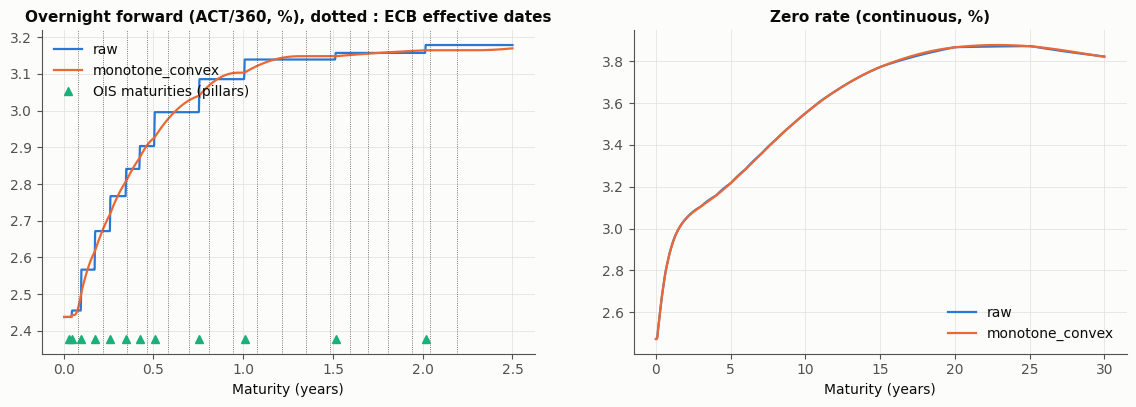
\includegraphics[width=\textwidth]{interpolation_comparison.png}
    \caption{Standard bootstrap. Left: overnight forward up to 2.5 years, with the ECB effective dates (dotted) and the OIS maturities (triangles). Right: zero rates.}
    \label{fig:interp}
\end{figure}

On the zero rates the two curves are indistinguishable (Figure~\ref{fig:interp}, right). The overnight forwards, however, show the problem of the short end (left):
\begin{itemize}
    \item \textbf{raw} jumps at the OIS maturities, i.e.\ at the pillars (triangles), dates on which nothing happens to the \estr{};
    \item \textbf{monotone convex} moves continuously and spreads each ECB decision over several months.
\end{itemize}
Neither reflects how the \estr{} actually moves: in steps, on the ECB effective dates (dotted lines). Both curves even let the forward rise before the first effective date, when no decision can change the \estr{}. This is the motivation of Section~\ref{sec:meetings}, which keeps the raw bootstrap for the long end and replaces the short end by steps on these dates.

\subsection{Validation of the bootstrap}
\label{sec:validation}
Repricing the input instruments with the functions used to build the curve is necessary but not sufficient, since an error shared by the bootstrap and the pricer (schedule, accrual, lag) cancels out. The curve is validated by the following tests.

\begin{enumerate}[label=(\arabic*)]
    \item \textbf{Repricing.} All quotes are repriced with a maximum residual of $1.1\times10^{-12}\bp$ (raw) and $6.6\times10^{-9}\bp$ (monotone convex), below the tolerance of $10^{-6}\bp$.
    \item \textbf{Independent implementation (QuantLib~\cite{quantlib}).} Two checks, with the same conventions (\texttt{Estr} index, \texttt{MakeOIS} / \texttt{OISRateHelper}, $T+2$, payment lag of one business day):
    \begin{itemize}
        \item our curves are passed to QuantLib as discount curves, and QuantLib prices the 25 OIS: its fair rates differ from our implied quotes by at most $2\times10^{-13}\bp$. The schedules coincide date by date (for instance the 18M OIS pays on 8 April 2027 and 10 April 2028 in both implementations), which validates the calendar, the stub, the day count and the payment lag;
        \item QuantLib bootstraps its own curve from the same quotes with log-linear discount factors, the equivalent of raw (\texttt{Piecewise\-Log\-Linear\-Discount}): over 30 years, its zero rates differ from ours by at most $2\times10^{-8}\bp$.
    \end{itemize}
    \item \textbf{Exact round trip.} Quotes are generated from a known curve whose pillars are the instrument maturities, then bootstrapped back with the same interpolation: the curve is recovered to $5\times10^{-11}\bp$ at the pillars and $1.4\times10^{-10}\bp$ on the instantaneous forwards over 30 years, for both methods.
    \item \textbf{Sanity checks.} The discount factors decrease strictly from $0.99993$ (one day) to $0.318$ (30 years), and the instantaneous forwards stay between $2.47\%$ and $4.25\%$ (continuously compounded, ACT/365; $2.47\%$ is today's \estr{} of $2.438\%$ ACT/360 in this convention).
    \item \textbf{Robustness.}
    \begin{itemize}
        \item The result does not depend on the order of the instruments (the bootstrapper sorts them by maturity).
        \item Starting the monotone convex solve from the raw solution shifted by $\pm50\bp$ or $+200\bp$ leads to the same curve within $2\times10^{-7}\bp$. The solver does not report convergence at its very strict tolerance ($10^{-15}$), which is why the bootstrap is checked on the residuals, not on the solver flag.
        \item A parallel $+1\bp$ shift of all quotes moves the zero curve by between $0.98$ and $1.01\bp$: par rates and zero rates do not move one for one.
        \item The sum of the par-point sensitivities equals the parallel sensitivity for raw, but not for monotone convex, which is not linear in its inputs (Section~\ref{sec:risk}).
    \end{itemize}
    \item \textbf{Out of sample (leave-one-out).} Each inner quote is removed in turn, the curve is rebuilt on the 24 others and the removed quote is repriced. The error has a root mean square of $1.42\bp$ for raw (maximum $3.6\bp$ on the 1M) and $0.32\bp$ for monotone convex (maximum $1.0\bp$ on the 1M). This favours monotone convex by construction, since the proxy quotes are generated from a smooth curve; with market quotes, which price a step path on the short end, the ranking could be different. The test comparing an OIS quote with the \estr{} realized afterwards requires historical OIS quotes and is left for real data.
\end{enumerate}

\begin{table}[htbp]
\centering
\footnotesize
\begin{tabular}{@{}lll@{}}
\toprule
Test & Criterion & Result \\
\midrule
Repricing & $\max|R_k|<10^{-6}\bp$ & $1.1\times10^{-12}$ (raw), $6.6\times10^{-9}$ (MC) bp \\
QuantLib pricing of our OIS & identical par rates & $\le2\times10^{-13}\bp$ \\
QuantLib bootstrap & identical curve & $\le2\times10^{-8}\bp$ on zero rates \\
Exact round trip & machine precision & $\le1.4\times10^{-10}\bp$ \\
Discount factors, forwards & decreasing, plausible & $0.318$--$0.99993$; $2.47$--$4.25\%$ \\
Order / starting point & identical curve & identical; $\le2\times10^{-7}\bp$ \\
Parallel $+1\bp$ & $\approx1\bp$ & $0.98$--$1.01\bp$ \\
Leave-one-out & within bid-ask & rms $1.42\bp$ (raw), $0.32\bp$ (MC) \\
\bottomrule
\end{tabular}
\caption{Validation tests of the standard \estr{} bootstrap (MC: monotone convex).}
\label{tab:validation}
\end{table}

\clearpage
% ===============================================================
\section{The Short End on ECB Meeting Dates}
\label{sec:meetings}
% ===============================================================

\subsection{Construction}
The overnight rate only moves materially on the ECB decision effective dates, and stays close to the deposit facility rate in between (Table~\ref{tab:spread}). A natural model of the short end is therefore a piecewise constant overnight forward with jumps on the effective dates $E_1<E_2<\dots$:
\begin{equation}
    f(0,t)=
    \begin{cases}
        r_{ON}, & t<E_1,\\
        f_k, & t\in[E_k,E_{k+1}),
    \end{cases}
    \label{eq:steps}
\end{equation}
with $f(0,\cdot)$ piecewise constant and $f(0,t)$ the instantaneous forward rate at time $t$, the pillars being placed on the meeting dates rather than on the instrument maturities. On $[0,E_1)$ the forward is today's fixing, known since no decision can change it before $E_1$. The jumps $f_{k}-f_{k-1}$ are the market-implied policy moves, and $(f_{k}-f_{k-1})/25\bp$ the implied number of $25\bp$ cuts or hikes.

The nodes are the effective dates up to a horizon of two years: 16 dates, from 4 November 2026 to 13 September 2028, hence 15 unknown levels $f_1,\dots,f_{15}$. The integrated forward at the nodes is
\begin{equation}
    y(E_1)=r_{ON}E_1,\qquad y(E_{k+1})=y(E_k)+f_k\,(E_{k+1}-E_k),
\end{equation}
and the curve between the nodes is the raw interpolation of the yield curve paper: linear in $y=-\ln P$, hence exactly the flat forwards of~\eqref{eq:steps}. No new interpolation is needed: only the position of the pillars changes.

\subsection{More meetings than quotes: penalty and choice of $\lambda$}
Only 11 OIS (1W to 18M) mature before the last node, for 15 unknown levels: the system is underdetermined, and infinitely many step paths reprice the short quotes. The levels are therefore obtained by least squares on the residuals (in basis points), with a penalty on the jumps,
\begin{equation}
    \min_{f_1,\dots,f_{15}}\ \sum_{k\in\text{short}}R_k^2+\lambda^2\sum_{k=1}^{15}\bigl(f_k-f_{k-1}\bigr)^2,\qquad f_0=r_{ON},
    \label{eq:penalty}
\end{equation}
with $\lambda=0.002$ (residuals and jumps in basis points). Among the paths that reprice the quotes, the penalty selects the one with the smallest jumps. Table~\ref{tab:lambda} shows the effect of $\lambda$:
\begin{itemize}
    \item with $\lambda=0$ the problem is ill-posed: the optimizer returns an oscillating path with $3{,}675\bp$ of cumulated jumps and $-31.5$ moves priced in one year;
    \item for $\lambda$ between $10^{-4}$ and $10^{-2}$ the solution does not change: the penalty only selects a path, and the residual of $0.79\bp$ does not come from $\lambda$ (Section~\ref{sec:residuals});
    \item from $\lambda\approx0.1$ the fit is traded for smoothness, and at $\lambda=1$ the curve no longer reprices the market ($5.4\bp$ of error).
\end{itemize}
The value $\lambda=0.002$ lies in the neutral region. A leave-one-out on the short quotes gives an optimum around $\lambda=0.03$ (root mean square error $0.52\bp$ against $0.57\bp$ at $\lambda=0.002$), a small difference which is moreover biased towards smoothing, since the proxy quotes come from a smooth curve. With market quotes, $\lambda$ would rather be chosen by the discrepancy principle: the largest value for which every quote stays repriced within its bid--ask.

\begin{table}[htbp]
\centering
\small
\begin{tabular}{@{}lrrrr@{}}
\toprule
$\lambda$ & Max residual (bp) & RMS residual (bp) & $\sum|f_k-f_{k-1}|$ (bp) & 25bp moves in 1 year \\
\midrule
0 & 0.785 & 0.254 & 3{,}675 & $-31.5$ \\
$10^{-4}$ to $10^{-2}$ & 0.785 & 0.254 & 72 & 2.72 \\
0.03 & 0.797 & 0.257 & 72 & 2.70 \\
0.1 & 0.870 & 0.289 & 72 & 2.70 \\
0.3 & 1.089 & 0.550 & 71 & 2.68 \\
1 & 5.358 & 2.564 & 65 & 2.42 \\
\bottomrule
\end{tabular}
\caption{Effect of the penalty $\lambda$ on the fit of the 11 short OIS and on the implied path.}
\label{tab:lambda}
\end{table}

The penalty also has a side effect: the levels beyond the last short maturity (18 months, April 2028) are constrained by no quote, so the penalty sets them equal to the previous one. The last four levels of Table~\ref{tab:ecb-path} (March to July 2028) are therefore identical, a plateau that is an artefact of the regularization, not market information.

\subsection{Long end}
Beyond the last node, each remaining OIS (2Y to 30Y) adds one pillar at its last payment date, with a flat forward from the previous pillar, solved sequentially with a one-dimensional root search: this is exactly the raw bootstrap of Section~\ref{sec:standard}. The whole curve is a single \texttt{YieldCurve} with raw interpolation on the union of the pillars (effective dates, then OIS maturities), and can be used directly by the pricers of the other papers.

\subsection{Residuals}
\label{sec:residuals}
The long quotes are repriced exactly (below $10^{-11}\bp$). The short ones are not quite: $0.79\bp$ on the 1M, $-0.27\bp$ on the 3M, $0.12\bp$ on the 4M, and less than $0.04\bp$ elsewhere. The 1M (end on 9 November) and the 2M (end on 7 December) OIS both end between the first two effective dates, and the forward before $E_1$ is fixed at today's \estr{}: a single level $f_1$ has to fit two quotes. The system is thus underdetermined overall but overdetermined locally. Proxy quotes generated from a smooth curve are not exactly compatible with a step path; market quotes, which already price a step path, would give much smaller residuals, and the remaining ones would measure the turn-of-month and turn-of-year effects that a richer curve would add as extra steps.

\begin{figure}[htbp]
    \centering
    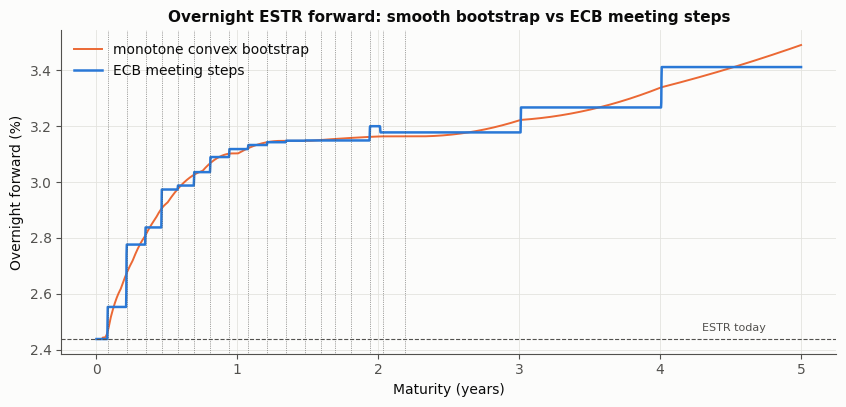
\includegraphics[width=\textwidth]{ecb_steps.png}
    \caption{Overnight \estr{} forward: monotone convex bootstrap vs ECB meeting steps.}
    \label{fig:ecb}
\end{figure}

\subsection{What changes with respect to the standard bootstrap}
Both constructions use the same quotes and differ only by where the overnight forward changes level: at the OIS maturities for the standard bootstrap, at the ECB effective dates for the meeting steps. Table~\ref{tab:compare} reads the overnight forward on a few dates around the first two effective dates.

\begin{table}[htbp]
\centering
\footnotesize
\begin{tabular}{@{}lrrrl@{}}
\toprule
Overnight forward (\%) on & Raw & Monotone convex & Meeting steps & \\
\midrule
20/10/2026 & 2.438 & 2.438 & 2.438 & today's \estr{} \\
03/11/2026 & 2.456 & 2.460 & 2.438 & day before $E_1$ \\
06/11/2026 & 2.456 & 2.476 & 2.553 & after $E_1$ (4/11) \\
12/11/2026 & 2.567 & 2.516 & 2.553 & after the 1M pillar \\
10/12/2026 & 2.672 & 2.627 & 2.553 & after the 2M pillar \\
28/12/2026 & 2.672 & 2.690 & 2.776 & after $E_2$ (23/12) \\
\midrule
Max $|\Delta r|$ vs steps, 0--2 years (bp) & 2.32 & 1.87 & -- & \\
Max $|\Delta P|$ vs steps, 0--2 years & $5.0\times10^{-5}$ & $4.0\times10^{-5}$ & -- & \\
Forward $E_1\to E_2$ (\%) & 2.590 & 2.585 & 2.557 & \\
\bottomrule
\end{tabular}
\caption{Standard bootstrap vs meeting steps on the same quotes (overnight forwards in ACT/360).}
\label{tab:compare}
\end{table}

Up to the first effective date the \estr{} cannot change: the meeting steps keep today's fixing, while raw and monotone convex already drift up. After it, the steps jump once and stay flat until the next decision, whereas raw jumps at the 1M and 2M payment dates. Discounting is barely affected (at most $2.3\bp$ on zero rates and $5\times10^{-5}$ on discount factors up to two years), but the forward between the first two meetings differs by about $3\bp$ with the same quotes: the construction matters for forward-starting instruments and for reading the policy path, not for plain discounting.

\subsection{Implied ECB policy path}
Each level $f_k$ is the \estr{} expected after a decision. Converted to an overnight ACT/360 rate and diminished by the current \estr{} $-$ DFR spread ($-6.3\bp$ over the last three months), it gives the implied deposit facility rate, and its change since today in units of $25\bp$ moves (Table~\ref{tab:ecb-path}).

\begin{table}[htbp]
\centering
\small
\begin{tabular}{@{}llrrrr@{}}
\toprule
Decision & Effective & \estr{} forward (\%) & Implied DFR (\%) & Change (bp) & 25bp moves \\
\midrule
29/10/2026 & 04/11/2026 & 2.553 & 2.616 & 11.5 & 0.46 \\
17/12/2026 & 23/12/2026 & 2.776 & 2.839 & 33.8 & 1.35 \\
04/02/2027 & 10/02/2027 & 2.838 & 2.900 & 40.0 & 1.60 \\
18/03/2027 & 24/03/2027 & 2.974 & 3.036 & 53.6 & 2.14 \\
29/04/2027 & 05/05/2027 & 2.988 & 3.051 & 55.0 & 2.20 \\
10/06/2027 & 16/06/2027 & 3.036 & 3.099 & 59.8 & 2.39 \\
22/07/2027 & 28/07/2027 & 3.090 & 3.153 & 65.2 & 2.61 \\
09/09/2027 & 15/09/2027 & 3.118 & 3.181 & 68.0 & 2.72 \\
28/10/2027 & 03/11/2027 & 3.133 & 3.196 & 69.5 & 2.78 \\
16/12/2027 & 22/12/2027 & 3.143 & 3.206 & 70.5 & 2.82 \\
03/02/2028 & 09/02/2028 & 3.148 & 3.211 & 71.0 & 2.84 \\
23/03/2028 & 29/03/2028 & 3.149 & 3.212 & 71.1 & 2.85 \\
04/05/2028 & 10/05/2028 & 3.149 & 3.212 & 71.1 & 2.85 \\
08/06/2028 & 14/06/2028 & 3.149 & 3.212 & 71.1 & 2.85 \\
20/07/2028 & 26/07/2028 & 3.149 & 3.212 & 71.1 & 2.85 \\
\bottomrule
\end{tabular}
\caption{Implied \estr{} forwards and deposit facility rate between ECB meeting dates (proxy quotes). Change and moves are measured from today's \estr{} of $2.438\%$.}
\label{tab:ecb-path}
\end{table}

On the proxy quotes, about $34\bp$ of hikes are priced by the end of 2026 and $71\bp$, i.e.\ 2.8 moves of $25\bp$, over 18 months; the moves are fractional because the forwards are expectations over the possible decisions. Three caveats apply. First, with proxy quotes this is the path implied by the AAA government curve, not by the OIS market. Second, risk-neutral forwards include a term premium, so they are not a forecast of the decisions. Third, the plateau of 2028 is set by the penalty, not by the data.

\subsection{Sensitivity to the proxy assumption}
\label{sec:proxy-sensitivity}
The proxy depends on the AAA--OIS basis $\bar b$. Table~\ref{tab:proxy-sensitivity} rebuilds the quotes and the meeting-step curve with the basis shifted by one standard deviation, and without basis.

\begin{table}[htbp]
\centering
\small
\begin{tabular}{@{}lrrrr@{}}
\toprule
Basis $\bar b$ & 2Y OIS (\%) & 5Y OIS (\%) & 10Y OIS (\%) & 25bp moves in 1 year \\
\midrule
$-13.8\bp$ (mean $-1$ std) & 3.1388 & 3.3065 & 3.6170 & 3.07 \\
$-4.9\bp$ (2-year mean) & 3.0521 & 3.2178 & 3.5281 & 2.72 \\
$+4.0\bp$ (mean $+1$ std) & 2.9654 & 3.1291 & 3.4392 & 2.37 \\
$0$ (no basis) & 3.0040 & 3.1686 & 3.4788 & 2.53 \\
\bottomrule
\end{tabular}
\caption{Proxy quotes and implied path for different AAA--OIS basis assumptions.}
\label{tab:proxy-sensitivity}
\end{table}

One standard deviation of the basis moves every OIS rate by about $9\bp$ and the number of moves priced in one year from 2.4 to 3.1. The basis acts almost as a parallel shift of the forwards beyond $E_1$, but since the first level is anchored on today's fixing, a parallel shift of the forwards becomes a change of the size of the first decisions. The construction is independent of the proxy; its levels are not, and market quotes are needed before reading anything economic into them.

\clearpage
% ===============================================================
\section{Risk: Par-Point Sensitivities}
\label{sec:risk}
% ===============================================================

The instrument is an 18-month $\times$ 4-year forward-starting receiver OIS: it receives a fixed rate of $3\%$ on a notional of EUR 10 million, from 18 months to 5.5 years, so its cash flows lie between the pillars. Its value on the meeting-step curve is $-127{,}475$ EUR, since the forward OIS rate is above $3\%$. Each quote is bumped by $+1\bp$ in turn, the curve rebuilt with the same construction and the trade repriced (Table~\ref{tab:risk}, Figure~\ref{fig:keyrates}).

\begin{table}[htbp]
\centering
\small
\begin{tabular}{@{}lrrr@{}}
\toprule
Quote bumped & Meeting steps & Monotone convex & Raw \\
\midrule
6M & $-8$ & $-7$ & $-7$ \\
1Y & 30 & 31 & 31 \\
18M & 1{,}429 & 1{,}436 & 1{,}427 \\
2Y & 33 & 15 & 34 \\
3Y & 6 & $-12$ & 6 \\
4Y & 14 & 225 & 14 \\
5Y & $-2{,}270$ & $-2{,}794$ & $-2{,}270$ \\
6Y & $-2{,}762$ & $-3{,}940$ & $-2{,}762$ \\
7Y & 0 & 403 & 0 \\
8Y & 0 & 2 & 0 \\
\midrule
Sum of par points & $-3{,}528$ & $-4{,}641$ & $-3{,}528$ \\
Parallel $+1\bp$ & $-3{,}526$ & $-3{,}527$ & $-3{,}526$ \\
\bottomrule
\end{tabular}
\caption{Par-point DV01 (EUR) of an 18m $\times$ 4y receiver OIS, EUR 10m (quotes with $|{\rm DV01}|>1$ EUR).}
\label{tab:risk}
\end{table}

\begin{figure}[htbp]
    \centering
    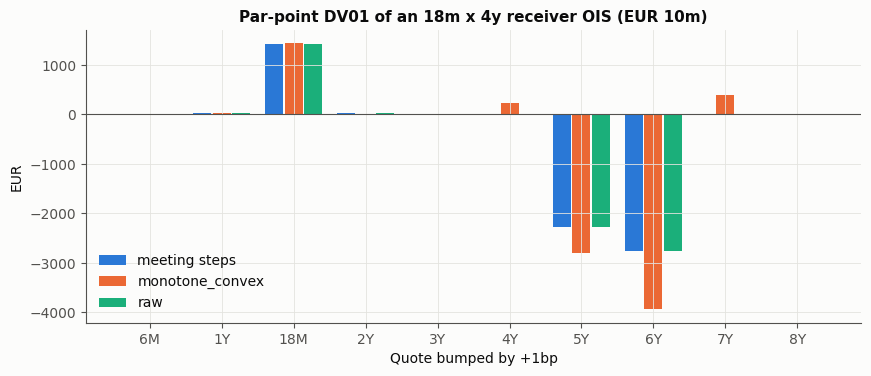
\includegraphics[width=\textwidth]{key_rates.png}
    \caption{Par-point DV01 of an 18m $\times$ 4y receiver OIS (EUR 10m).}
    \label{fig:keyrates}
\end{figure}

The parallel DV01 is the same for the three constructions, about $-3{,}527$ EUR per basis point: a receiver loses when rates rise. Its split across the quotes shows three things.
\begin{itemize}
    \item The risk sits on the quotes that bracket the flows: the 18M quote, at the start of the swap ($+1{,}429$ EUR: a higher 18M rate lowers $P(0,18\mathrm{M})$ and the value of the floating leg that the receiver pays), and the 5Y and 6Y quotes, around its end at 5.5 years ($-2{,}270$ and $-2{,}762$ EUR).
    \item \textbf{Meeting steps and raw give the same risk.} Both have flat forwards between their pillars, and the flows of the trade start after the last meeting node (18 months), where both curves are built the same way.
    \item \textbf{Monotone convex spreads the risk} on the 4Y and 7Y quotes ($+225$ and $+403$ EUR), and its par-point DV01s add up to $-4{,}641$ EUR against a parallel DV01 of $-3{,}527$ EUR. The method is not linear in its inputs (its forward constraints switch regions when a quote moves, as in the yield curve paper), so its bucketed risk is not additive. This is a practical argument for flat forwards on a risk curve, on top of the monetary policy argument of Section~\ref{sec:meetings}.
\end{itemize}
Bumping and rebuilding costs one bootstrap per quote; the bootstrap Jacobian, $\partial z/\partial q=-(\partial_zR)^{-1}\partial_qR$, would give all the sensitivities at once (Section~\ref{sec:next-steps}).

\clearpage
% ===============================================================
\section{Limitations}
\label{sec:limits}
% ===============================================================

\paragraph{Proxy quotes.} The levels of the curve come from the AAA government curve, shifted by a basis measured ex post at three months only, which mixes the basis with forecast errors and has varied by tens of basis points since 2019 (down to $-100\bp$ in 2022). The same constant basis is applied at every maturity, and the quotes below three months are generated by the model. One standard deviation of the basis moves the OIS rates by $9\bp$ and the policy path by 0.35 moves in one year.

\paragraph{Data.} The curve is built on a single valuation date, from mid quotes; the bid--ask spread, which would be the natural tolerance of the fit and of the choice of $\lambda$, is ignored.

\paragraph{Conventions.} The conventions match QuantLib's \estr{} OIS, but the holiday calendar is stored from 2019 to 2060 only, and the rounding rules of the compounded rate in real confirmations are not reproduced.

\paragraph{Short end.} The meeting-step model assumes that the \estr{} does not move between two decisions, and that the \estr{} $-$ DFR spread is constant; turn-of-month and turn-of-year effects are not modelled. The choice of $\lambda$ and of the two-year horizon is ad hoc, and the levels beyond the last short quote are set by the penalty.

\paragraph{Long end.} The forward is flat beyond the last quote (30 years). Long-dated \estr{} OIS are also less liquid than EURIBOR swaps, so with real data the long end would rather be built from EURIBOR swaps and \estr{}/EURIBOR basis swaps.

\paragraph{Collateral.} \estr{} discounting assumes cash collateral in euros remunerated at \estr{}; other collateral agreements (USD collateral, no CSA) require other discount curves.

% ===============================================================
\section{Next Steps}
\label{sec:next-steps}
% ===============================================================

\begin{itemize}
    \item Use real quotes: fill \texttt{ESTR\_OIS\_Quotes\_YYYYMMDD.csv}, and add meeting-date OIS, which pin down each level of the short end directly.
    \item Choose $\lambda$ and the horizon of the meeting nodes by the discrepancy principle, with the residuals normalized by the bid--ask of each quote.
    \item Gather the code in an \texttt{EstrCurveBuilder} class (TARGET calendar, \estr{} index, instruments, quote source, builder) returning a \texttt{YieldCurve}, with the policy path and the par-point risk as methods.
    \item Compute the risk with the bootstrap Jacobian instead of bumping and rebuilding.
    \item Build the EURIBOR 3M and 6M projection curves on \estr{} discounting (multi-curve framework).
    \item Calibrate Hull--White on \estr{} discounting and price the callable range accrual and Bermudan swaptions.
    \item Rebuild the curve every day and study its principal components, as in the yield curve paper.
    \item Cross-currency: SOFR curve and EUR/USD basis.
\end{itemize}

% ===============================================================
\section{Conclusion}
\label{sec:conclusion}
% ===============================================================

The \estr{} curve is the discount curve of collateralized euro derivatives. This paper builds it from public data, with the market conventions of \estr{} OIS. The conventions are validated twice: the ECB compounded index is rebuilt from 1,797 fixings to $5\times10^{-9}$, and the OIS priced on our curve match QuantLib to $2\times10^{-13}\bp$, with identical schedules.

A standard bootstrap, with one pillar per OIS, reprices the 25 quotes exactly and is independently reproduced by QuantLib, but its overnight forwards do not move like the \estr{}: they jump at the OIS maturities (raw) or spread each decision over several months (monotone convex). Placing the short-end pillars on the ECB effective dates gives a step path, flat between decisions, from which the expected policy can be read directly: on the proxy quotes, 2.8 hikes of $25\bp$ are priced over 18 months. Both constructions discount almost identically, within $2.3\bp$ of zero rate, but differ by $3\bp$ on a forward between two meetings, and the flat-forward constructions give additive bucketed risks, which monotone convex does not.

The main limit is the data: without free OIS quotes, the levels of the curve come from the AAA government curve and an estimated basis, whose uncertainty of one standard deviation moves the implied path by 0.35 hikes in one year. The construction itself is independent of this proxy, and with market quotes only the input file changes.

\clearpage

% ===============================================================
\appendix
\section{Python Implementation (Excerpts)}
\label{app:code}
% ===============================================================

The following listings are excerpts of the implementation (package \texttt{Fixed\_Income\_Models} and notebook \texttt{estr\_curve.ipynb}), slightly simplified. The full scripts and the notebook are available on GitHub.

\subsection{Dated \texteuro STR OIS}
\begin{lstlisting}[style=pystyle]
class OIS(Instrument):
    # Spot-starting ESTR OIS with a dated schedule ; maturity (pillar) = last payment time
    def __init__(self, tenor, rate, spot=SPOT, pay_lag=1):
        end = add_tenor(spot, tenor)
        months = ...                                   # tenor in months (0 for weeks)
        ends, k = [end], 12
        while months - k > 0:                          # annual periods, short front stub
            ends.insert(0, modified_following(spot + pd.DateOffset(months=months - k)))
            k += 12
        starts = [spot] + ends[:-1]
        pays = [roll(e, pay_lag) for e in ends]        # payment 1 business day after each end
        self.t_start, self.t_end, self.t_pay = time(starts), time(ends), time(pays)
        self.accrual = np.array([(e - s).days / 360 for s, e in zip(starts, ends)])
        super().__init__(self.t_pay[-1], rate)

    def implied_quote(self, curve):
        P_pay = curve.discount(self.t_pay)
        floating = np.sum(P_pay * (curve.discount(self.t_start) / curve.discount(self.t_end) - 1))
        return floating / np.sum(self.accrual * P_pay)
\end{lstlisting}

\subsection{Proxy quotes}
\begin{lstlisting}[style=pystyle]
def proxy_curve(basis_bp=BASIS_BP):
    # ESTR flat until the first effective date, then AAA forward minus the basis
    grid = np.unique(np.concatenate([[FIRST_EFFECTIVE], np.linspace(FIRST_EFFECTIVE, 32, 600)]))
    h = 1e-4
    aaa_y = lambda t: svensson(t, *row[SVENSSON]) / 100 * t
    fwd = (aaa_y(grid + h) - aaa_y(grid - h)) / (2 * h) - basis_bp * 1e-4
    y = ON * FIRST_EFFECTIVE + np.concatenate([[0.0], np.cumsum(0.5 * (fwd[1:] + fwd[:-1]) * np.diff(grid))])
    return YieldCurve(grid, y / grid, "linear_zero")

quotes = [OIS(t, 0.0) for t in TENORS]
for q in quotes:
    q.quote = q.implied_quote(proxy_curve())
\end{lstlisting}

\subsection{Meeting-step curve}
\begin{lstlisting}[style=pystyle]
def meeting_curve(quotes, effective_times, horizon=2.0, penalty=0.002):
    nodes = np.array([e for e in effective_times if e <= horizon])        # E_1 < ... < E_n
    short = [q for q in quotes if q.maturity <= nodes[-1]]
    long = [q for q in quotes if q.maturity > nodes[-1]]

    def build(levels):
        # forward ON on [0, E_1), levels[k] on [E_{k+1}, E_{k+2}) : raw interpolation of y
        y = ON * nodes[0] + np.concatenate([[0.0], np.cumsum(levels * np.diff(nodes))])
        return YieldCurve(nodes, y / nodes, "raw"), y

    def residuals(levels):
        c, _ = build(levels)
        fit = [1e4 * q.residual(c) for q in short]
        jumps = penalty * 1e4 * np.diff(np.concatenate([[ON], levels]))
        return np.concatenate([fit, jumps])

    sol = least_squares(residuals, np.full(len(nodes) - 1, ON))
    _, y = build(sol.x)
    times, zeros = list(nodes), list(y / nodes)
    for q in long:                                   # long end : one pillar per OIS, flat forward
        f = lambda z: q.residual(YieldCurve(np.array(times + [q.maturity]), np.array(zeros + [z]), "raw"))
        zeros.append(brentq(f, -0.05, 0.2, xtol=1e-14)); times.append(q.maturity)
    return YieldCurve(np.array(times), np.array(zeros), "raw"), pd.Series(sol.x, index=nodes[:-1]), short
\end{lstlisting}

\section{Notation}
\label{app:notation}

\begin{table}[h]
\centering
\begin{tabular}{@{}lp{11.5cm}@{}}
\toprule
Symbol & Meaning \\
\midrule
$r_i,\ n_i$ & \estr{} fixing of business day $d_i$ and number of calendar days to the next business day \\
$R(T_s,T_e)$ & Daily compounded \estr{} over $[T_s,T_e]$ \\
$I_t$ & ECB compounded \estr{} index \\
$P(0,T),\ y(T)$ & \estr{} discount factor and integrated forward $-\ln P(0,T)$ \\
$T_0$ & Spot date (valuation date $+2$ business days) \\
$s_i,\ e_i,\ p_i,\ \tau_i$ & Start, end and payment dates of period $i$, ACT/360 accrual \\
$S(T),\ K$ & \estr{} OIS par rate \\
$r_0,\ r_{ON}$ & Today's \estr{} fixing, and its continuously compounded ACT/365 equivalent \\
$z_{\mathrm{AAA}},\ f_{\mathrm{AAA}}$ & AAA Svensson spot rate and instantaneous forward \\
$b(t),\ \bar b$ & Ex-post AAA--\estr{} basis and its 2-year mean \\
$E_k,\ f_k$ & ECB decision effective dates and overnight forwards on $[E_k,E_{k+1})$ \\
$\lambda$ & Penalty on the jumps of the meeting-step forwards \\
$q_k,\ R_k,\ z$ & Market quotes, residuals and bootstrap unknowns \\
\bottomrule
\end{tabular}
\caption{Main notation.}
\label{tab:notation}
\end{table}

\clearpage

% ===============================================================
\begin{thebibliography}{99}
% ===============================================================

\bibitem{data}
ECB data,
\textit{\url{https://data.ecb.europa.eu}}

\bibitem{haganwest2006}
P. S. Hagan and G. West,
\textit{Interpolation methods for curve construction},
Applied Mathematical Finance, 13(2):89--129, 2006.

\bibitem{ametrano}
F. M. Ametrano and M. Bianchetti,
\textit{Everything you always wanted to know about multiple interest rate curve bootstrapping but were afraid to ask},
SSRN Working Paper 2219548, 2013.

\bibitem{henrard}
M. Henrard,
\textit{Interest Rate Modelling in the Multi-Curve Framework},
Palgrave Macmillan, 2014.

\bibitem{andersenpiterbarg}
L. B. G. Andersen and V. V. Piterbarg,
\textit{Interest Rate Modeling, Volume I: Foundations and Vanilla Models},
Atlantic Financial Press, 2010.

\bibitem{ecbestr}
European Central Bank,
\textit{Euro short-term rate (\texteuro STR) methodology and policies},
Available at: \url{https://www.ecb.europa.eu/stats/financial_markets_and_interest_rates/euro_short-term_rate/html/index.en.html}

\bibitem{ecbdata}
European Central Bank,
\textit{ECB Data Portal},
Available at: \url{https://data.ecb.europa.eu}

\bibitem{quantlib}
\textit{QuantLib, a free/open-source library for quantitative finance},
Available at: \url{https://www.quantlib.org}

\bibitem{yieldcurve}
E. Benguedda,
\textit{Yield Curve Construction: Interpolation, Bootstrapping and Curve Risk},
2026. Available on the portfolio: \url{https://portfolio-eliasbenguedda.fr}

\bibitem{svensson}
L. E. O. Svensson,
\textit{Estimating and interpreting forward interest rates: Sweden 1992--1994},
NBER Working Paper 4871, 1994.

\end{thebibliography}

\end{document}
